\documentclass[../user-manual.tex]{subfiles}

\begin{document}
	
	В данной главе рассматриваются вопросы создания и редактирования объектов системы Магрепорт, используемых для получения доступа к данным и формирования отчётов. Все примеры построены на открытой базе данных численности населения населённых пунктов Российской Федерации, размещённой на Платформе ИНИД по адресу:
	
	\begin{boxed}
		https://www.data-in.ru/data-catalog/datasets/160
	\end{boxed}
	
	Вы можете загрузить этот набор данных в свою БД и проделать все описанные ниже шаги для построения учебного примера. В примерах таблица была обогощена значением кодов регионов. На основе таблицы были созданы представления для справочников регионов, муниципалитетов, типов поселений и самих поселений. Префиксом <<F\_>> мы традиционно обозначем представления фактов, префиксом <<R\_>> --- представления справочников.
	
	\begin{concept}
		Магрепорт мог бы использовать одну и ту же исходную таблицу фактов и для создания всех необходимых фильтров, так как он добавляет при запросе к справочникам при обращении из фильтров группировку до нужного уровня. Однако мы специально создали для всех интересующих нас бизнес-сущностей отдельные справочные представления по следующим причинам:
		
		\begin{itemize}
			\item В реальном примере скорее всего существовали бы отдельные таблицы для справочников, так как таблица фактов, как правило, имеет временной разрез и слишком громоздка, чтобы было допустимо на лету вычислять по ней справочную информацию путём группировки.
			
		\end{itemize}
	\end{concept}
	
	\begin{boxed}

		\begin{itemize}

		
		\item Если даже есть соблазн всё сделать на одной денормализованной таблице, лучше отдельно выделить хотя бы в виде представлений справочники бизнес-сущностей, во-первых, в целях создания качественной модели данных, а во-вторых, чтобы для Магрепорта разграничить пулы коннектов к фактам и справочникам (хотя, конечно, можно дважды добавить одну и ту же таблицу через разные источники данных, но это может привести к путанице) --- Магрепорт ограничивает количество одновремеменно выполняющихся запросов для каждого источника данных и хорошей практикой является изоляция пулов быстрых и медленных запросов.
		\end{itemize}
	\end{boxed}

	Общая для всех типов объектов кнопка создания объектов расположена в правом нижнем углу окна приложения (см. рис. \ref{fig:create-object-button}). При помощи этой же кнопки создаются каталоги для размещения объектов. Создать объект вне каталога на самом верхнем уровне иерархии каталогов (то есть в корневом каталоге) нельзя.
	
	Вход в мастер редактирования объектов осуществляется путём нажатия кнопки <<Редактировать>> в окне просмотра объекта (вызывается для большинства объектов путём нажатия на карточку объекта, для отчётов --- через нажатие кноки <<Просмотр>> на карточке объекта) или кнопки <<Редактировать>> в виде карандаша на карточке объекта.
	
	Некоторые атрибуты объектов не могут быть отредактированы --- в частности набор данных отчёта, поскольку изменение набора данных, лежащего в основе отчёта равносильно созданию нового отчёта. Некоторые атрибуты не могут быть заданы при создании объекта --- могут быть добавлены только при редактировании, в частности шаблоны отчётов.
	

	\begin{figure}[h]
		\centering
		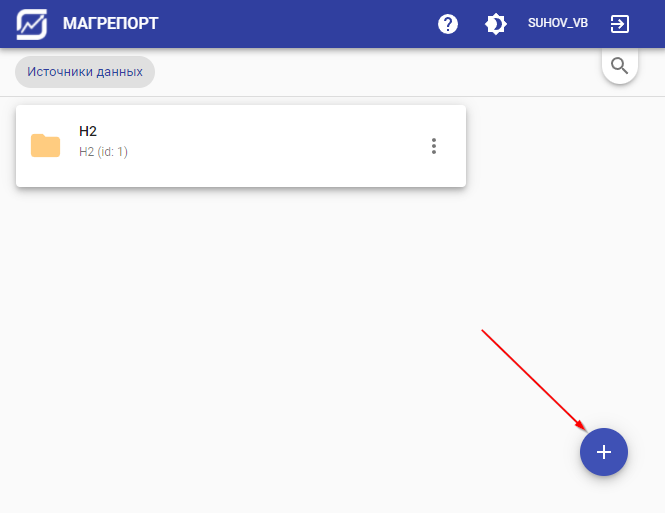
\includegraphics[width=\graphicswidth]{img/1-create-object-button.png}
		\caption{Кнопка создания объектов}
		\label{fig:create-object-button}
	\end{figure}

	Конечным целевым продуктом разработки в системе Магрепорт является сущность <<Отчёт>> --- именно эти объекты используются конечным пользователем для получения данных. Сущность <<Отчёт>> в свою очередь использует в своём дизайне сущности <<Набор данных>> и <<Фильтр>> для, соответственно, получения данных и управления фильтрацией. Сущность <<Фильтр>> также может использовать в своём дизайне сущность <<Набор данных>>, если фильтр основан на справочнике. Наконец, сущность <<Набор данных>> использует базовую сущность <<Источник данных>> для обращения к СУБД. Ниже описаны процессы разработки всех этих сущностей.
	
	Все разрабатываемые объекты могут быть скопированы или перенесены в рамках каталогов, на которые данный разработчик имеет права записи.

	
	\section{Создание источников данных}\label{developing:datasources}
	
	Для доступа к БД необходимо создать объект подключения, называемый в Магрепорте \textit{источником данных}. Для создания объекта источника данных необходимо перейти в раздел <<Разработка / Источники данных>> (через соответствующий пункт бокового меню), создать соответствующую потребностям структуру каталогов и создать в них объекты источников данных (см. рис. \ref{fig:create-datasource}).
	
	\begin{figure}[h]
		\centering
		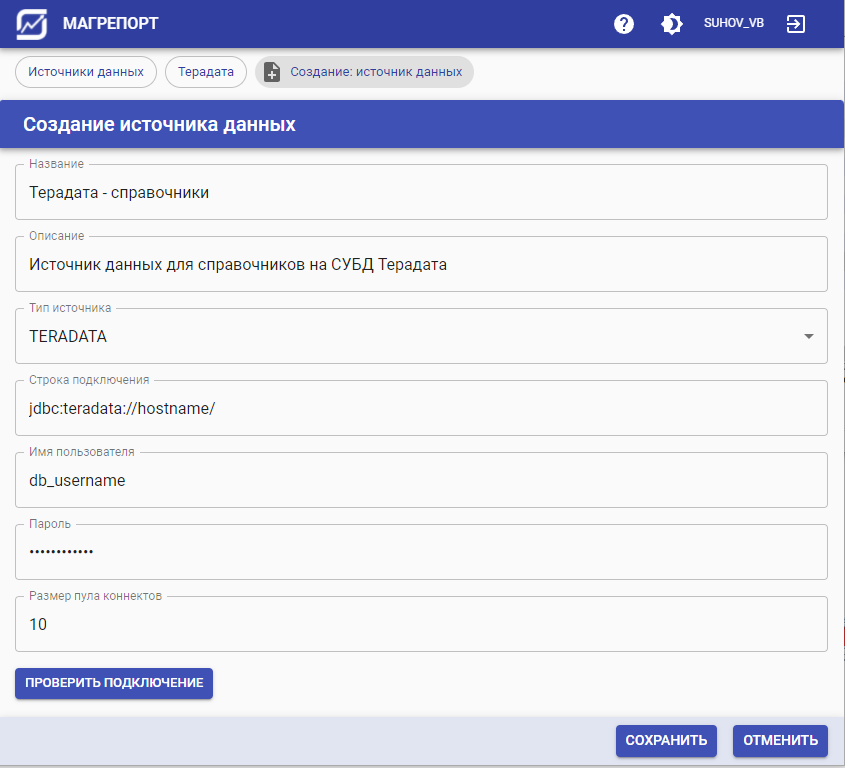
\includegraphics[width=\graphicswidth]{img/2-create-datasource.png}
		\caption{Дизайнер объектов <<Источник данных>>}
		\label{fig:create-datasource}
	\end{figure}

	Названия параметров создаваемого подключения (источника данных) достаточно точно отражают их предназначение. Отметим некоторые важные особенности создания и редактирования подключения:
	
	\begin{itemize}
		\item \textbf{Тип источника} определяет тип СУБД, для которой создаётся подключение. Абстрактного универсального подключения нет. Список поддерживаемых типов СУБД является расширяемым в новых версиях Магрепорта. Если интересующей вас СУБД не оказалось в списке, вы можете связаться с командой разработки системы Магрепорт по вопросы добавления соответствующего коннектора.
		
		\item \textbf{Строка подключения} Указывается строка jdbc-подключения к СУБД. Файл с соответствующим jdbc-драйвером должен быть размещён в каталоге jdbc домашнего каталога Магрепорт (домашним считается каталог размещения исполняемого файла magreport.jar). В комплект поставки Магрепорта входят jdbc-драйверы некоторых СУБД определённых версий. Их можно заменить на более свежие версии.
		
		\item \textbf{Имя пользователя} и \textbf{пароль} --- имя и пароль пользователя СУБД, используемые для данного подключения. <<Проброс>> имени и пароля пользователя Магрепорт в СУБД не предусмотрен. При редактировании параметров подключения необходимо заново вводить пароль пользователя --- иначе он будет перезаписан пустым.
		
		\item \textbf{Размер пула коннектов} Максимальное количество одновременно выполняющихся запросов для данного подключения. При отсутствии свободных подключений запросы становятся в очередь. Запросы из очереди попадают на выполнение при освобождении коннектов в порядке постановки в очередь.
		
	\end{itemize}

	\begin{concept}
		Разработчики Магрепорт не реализовали возможность <<проброса>> имени и пароля текущего пользователя в качестве пользователя СУБД, во-первых, из нежелания сохранять где-либо пароль пользователя, а, во-вторых, что даже важнее, из убеждённости, что такая практика приводит к чрезмерно сложной системе разграничения прав доступа --- ральные права пользователя в таком случае являются пересечением его прав на уровне истсемы отчётности и на уровне СУБД. Разобраться в такой системе на каком уровне произошёл отказ доступа становится очень сложно, как и поддерживать целостность такой системы. Разработчики Магрепорт уверены, что механизмы управления правами доступа в системе Магрепорт достаточно развитые, гибкие и удобные, чтобы при помощи них можно было решить все задачи обспечения информационной безопасности при работе с данными. 
	\end{concept}

	\begin{NB}
		Обратите внимание, что при редактировании источника данных необходимо заново указывать пароль пользователя СУБД.
	\end{NB}

	\begin{adminnote}
		Для добавления необходимых JDBC-драйверов нужно соответствующие jar-файлы разместить в каталоге jdbc домашнего каталога системы Магрепорт. Потенциально конфликтующие jar-файлы (содержащие тот же драйвер, но другой версии) при этом стоит оттуда удалить.
	\end{adminnote}

	\begin{concept}
		Каждый источник данных имеет ограничение на размер пула коннектов. Такое ограничение позволяет контролировать использование ресурсов сервера Магрепорта и сервера СУБД. С учётом ограниченного пула коннектов крайне полезно бывает разграничить пулы для медленных и быстрых запросов (либо ввести ещё более разветвлённую градацию). К быстрым запросам относятся запросы к справочникам сущностей, которые в процессе своей работы осуществляют фильтры. Такие запросы не должны конкурировать с медленными запросами на выполнение отчётов, поэтому рекомендуется для каждой СУБД, которая используется и для справочников и для конечных отчётов, создавать по крайней мере два объекта источника данных.
	\end{concept}

	\begin{concept}
		В Магрепорте не реализовано кэширование справочных данных, которое можно встретить в некоторых других системах отчётности. Разработчики Магрепорта считают, что это усложняет использование системы необходимостью управлять синхронизацией кэшей и добавляет ей непрофильный функционал, который гораздо более успешно можно реализовать на уровне СУБД.
	\end{concept}
		

	При создании и редактировании источника данных есть возможность проверить корректность задания параметров при помощи тестового подключения к СУБД, воспользовавшись кнопкой <<Проверить подключение>>.
		
	\section{Создание наборов данных}
	
	Для доступа к конкретной таблице, представлению или хранимой процедуре БД в Магрепорте используется сущность <<Набор данных>>. Для создания объекта набора данных необходимо перейти в раздел <<Разработка / Наборы данных>> (через соответствующий пункт бокового меню), создать соответствующую потребностям структуру каталогов и создать в них объекты наборов данных (см. рис. \ref{fig:create-dataset}).
	
	\begin{figure}[h]
		\centering
		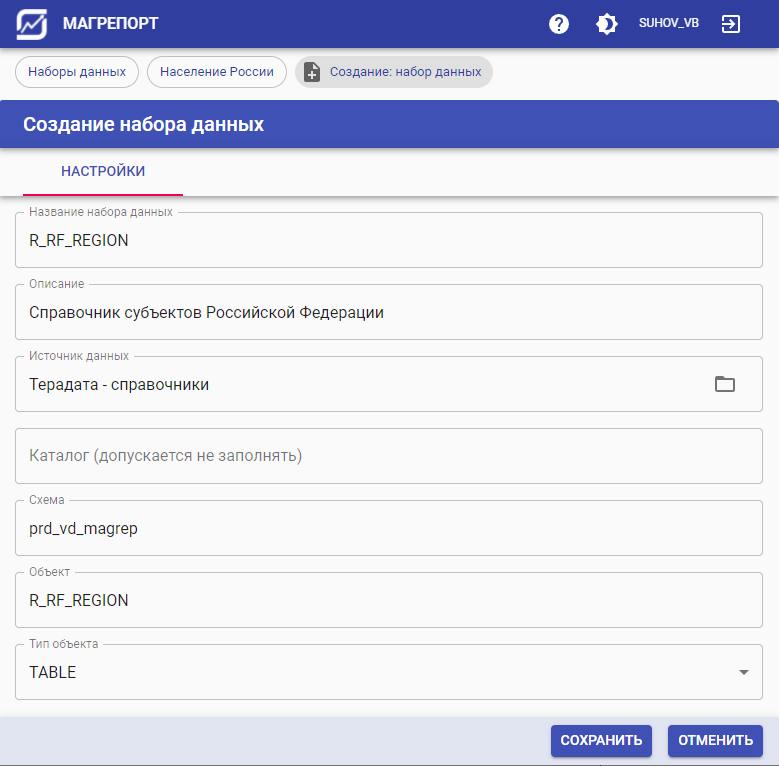
\includegraphics[width=\graphicswidth]{img/3-create-dataset.png}
		\caption{Дизайнер объектов <<Набор данных>>}
		\label{fig:create-dataset}
	\end{figure}

	При создании набора данных нужно задать следующие параметры:
	
	\begin{itemize}
		\item \textbf{Название набора данных} Название создаваемого объекта в Магрепорте (разработчик может назвать объект набора данных произвольным образом, не обязательно связанным с названием объекта в БД).
		
		\item \textbf{Описание} Описание набора данных.
		
		\item \textbf{Источник данных} Нажав на кнопку в виде папки в строке поля, необходимо выбрать  источник данных, который будет использоваться для подключения к БД.
		
		\item \textbf{Каталог} Для некоторых СУБД существует такой уровень иерархии объектов, как каталог. Для таких СУБД необходимо указать каталог, для остальных поле нужно оставить пустым.
		
		\item \textbf{Схема} Схема СУБД, в которой расположен добавляемый объект БД.
		
		\item \textbf{Объект} Название добавляемой таблицы, представления или хранимой процедуры.
		
		\item \textbf{Тип объекта} Для таблиц и представлений указывается <<TABLE>>. Для отчётов на хранимых процедурах указывается <<PROCEDURE>>. 
	
	\end{itemize}

	\begin{modelExample}
		В модельном примере мы создадим следующие наборы данных:
		\begin{itemize}
			\item \textbf{R\_RF\_REGION} --- справочник субъектов Российской Федерации. Поля:
				\begin{itemize}
					\item \textbf{region\_code} --- код субъекта
					\item \textbf{region\_name} --- название субъекта
				\end{itemize}
			
			\item \textbf{R\_MUNICIPALITY} --- справочник муниципальных образований Российской Федерации. Поля:
				\begin{itemize}
					\item \textbf{region\_code} --- код субъекта
					\item \textbf{region\_name} --- название субъекта
					\item \textbf{municipality} --- название муниципального образования
				\end{itemize}
						
			\item \textbf{R\_SET\_TYPE} --- справочник типов населённых пунктов. Поля:
				\begin{itemize}
					\item \textbf{set\_type} --- сокращённое обозначение типа населённого пункта
					\item \textbf{set\_type\_name} --- полное наименование типа населённого пункта
				\end{itemize}			
			
			\item \textbf{R\_SETTLEMENT} --- справочник типов населённых пунктов. Поля:
				\begin{itemize}
					\item \textbf{settlement\_id} --- ID населённого пункта
					\item \textbf{region\_code} --- сокращённое обозначение типа населённого пункта
					\item \textbf{region\_name} --- полное наименование типа населённого пункта
					\item \textbf{municipality} --- название муниципального образования
					\item \textbf{set\_type} --- сокращённое обозначение типа населённого пункта
					\item \textbf{settlement} --- название населённого пункта
					\item \textbf{oktmo} --- код ОКТМО населённого пункта
					\item \textbf{latitude\_dms}, \textbf{longitude\_dms}, \textbf{latitude\_dd}, \textbf{longitude\_dd} --- географические координаты (долгота и широта) населённого пункта в различных системах
				\end{itemize}
			
			\item \textbf{F\_SETTLEMENTS\_STATS} --- таблица численности населения населённых пунктов Российской Федерации (см. в начале главы).
			
		\end{itemize}
	\end{modelExample}

	\begin{concept}
		Магрепорт не выполняет JOIN таблиц при формировании запросов к БД, поэтому таблицы (или представления) следует создавать денормализованными (как таблицы фактов, так и справочники).
	\end{concept}
	
	\section{Создание фильтров}\label{developing:filters}
	
	Фильтрами называются объекты системы Магрепорт, позволяющие пользователю задавать фильтрацию запроса к БД --- результат взаимодействия пользователя с фильтрами есть предикат SQL-запроса (секция WHERE). Для создания фильтра необходимо перейти в раздел <<Разработка / Экземпляры фильтров>> (через соответствующий пункт бокового меню), создать соответствующую потребностям структуру каталогов и создать в них объекты экземпляров фильтров (см. рис \ref{fig:create-filter-instance}).
	
	\begin{concept}
		В системе Магрепорт есть несколько сущностей, в названии которых присутствует слово <<фильтр>>. Это \textit{шаблоны фильтров}, \textit{экземпляры фильтров}, \textit{фильтры безопасности} и \textit{фильтры в отчёте}. \textit{Шаблоны фильтров} --- это системные объекты, которые задают принципы конструирования и поведения \textit{экземпляров фильтров}, построенных на них. Например, шаблоном фильтра является абстрактный иерархический фильтр, позволяющий пользователю делать выбор в иерархическом дереве. \textit{Экземпляр фильтра} в свою очередь задаёт конкретную реализацию фильтра. Например, иерархический фильтр по населённым пунктам является реализацией абстрактного шаблона иерархического фильтра. \textit{Фильтры безопасности} --- специальные объекты, позволяющие на основе экземпляров фильтров управлять правами пользователей на уровне данных (подробнее фильтры безопасности рассматриваются в главе \ref{administration}). \textit{Фильтры в отчёте} --- это не совсем самостоятельные сущности, а фактически связь отчёта и экземпляра фильтра, наделённая, возможно, дополнительными атрибутами.
	\end{concept}

	\begin{figure}[h]
		\centering
		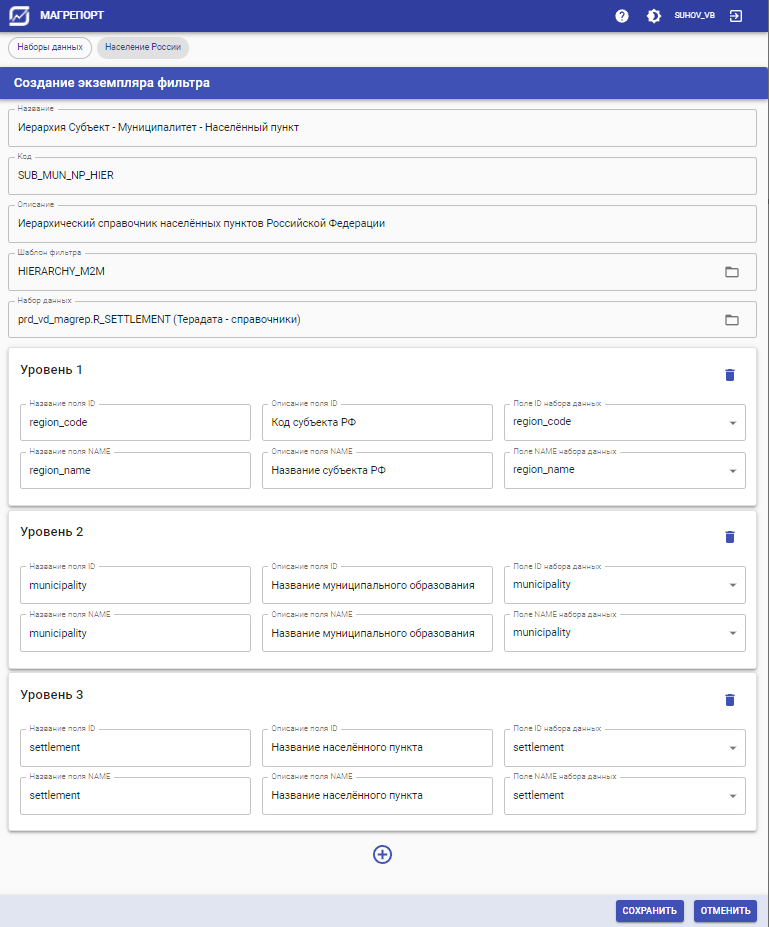
\includegraphics[width=\graphicswidth]{img/4-create-filter-instance.png}
		\caption{Дизайнер объектов <<Экземпляр фильтра>>}
		\label{fig:create-filter-instance}
	\end{figure}

	При создании экземпляра фильтра требуется задать значения следующих атрибутов:
	
	\begin{itemize}
		
		\item \textbf{Название} --- название экземпляра фильтра.
		
		\item \textbf{Код} --- символьный код, используемый по умолчанию в качестве кода фильтров в отчёте. Код фильтра в отчёте используется при получении значений фильтров в отчётах на базе хранимых процедур. Если вы не используете отчёты на базе хранимых процедурах, код фильтра вам не понадобится (однако он является обязательным полем). Подробнее создание отчётов на базе хранимых процедур рассмотрено в разделе \ref{developing:stored-procedure-reports}.
		
		\item \textbf{Описание} --- описание экземпляра фильтра.
		
		\item \textbf{Шаблон фильтра} --- указывается шаблон фильтра, на основе которого создаётся экземпляр фильтра.
		
	\end{itemize}

	Состав остальных атрибутов экземпляра фильтра зависит от шаблона фильтра. Ниже будут подробнее рассмотрены существующие шаблоны фильтров. Все шаблоны фильтров условно деляться на два класса: использующие таблицы-справочники БД, и не использующие их. Экземпляры фильтров на основе шаблонов первого типа требуют указания набора данных и указания его полей, из которых фильтр должен получать данные.
	
	Все шаблоны фильтров собраны в системной папке <<Дефолтные шаблоны фильтров>> раздела <<Разработка / Шаблоны фильтров>>, недоступной для редактирования. Ниже описаны существующие шаблоны фильтров.
	
	\begin{itemize}
		\item \textbf{SINGLE\_VALUE\_UNBOUNDED} --- при помощи данного фильтра пользователю предоставляется возможность указать конкретное значение, не ограниченное никаким справочником. Данное значение используется для фильтрации по выбранному полю отчёта по условию равенства (\textit{поле} \textbf{=} \textit{значение}). На настоящий момент не реализованы другие условия (неравенство, больше, меньше и др.), но в следующих версиях их планируется добавить.
		
		\item \textbf{RANGE} --- при помощи данного фильтра пользователю предоставляется возможность указать диапазон значений. Этот диапазон используется для фильтрации по выбранному полю отчёта по условию \textbf{BETWEEN} (\textit{поле} \textbf{BETWEEN} \textit{начальное значение} \textbf{AND} \textit{конечное значение}). На настоящий момент не реализовано условие \textbf{NOT BETWEEN}, его реализацию планируется добавить в следующих версиях.
		
		\item \textbf{VALUE\_LIST\_UNBOUNDED} --- при помощи данного фильтра пользователю предоставляется возможность указать несколько значений (через разделитель --- пробел, запятую, точку с запятой), не ограниченных никаким справочником. Данные значения используются для фильтрации по выбранному полю отчёта по условию включения в список (\textit{поле} \textbf{IN} \textbf{(} \textit{значение 1}, \textit{значение 2}, \textit{значение 3}, ... \textbf{)}). На настоящий момент не реализовано условие \textbf{NOT IN}, его реализацию планируется добавить в следующих версиях.
		
		\item \textbf{VALUE\_LIST} --- при помощи данного фильтра пользователю предоставляется возможность указать несколько значений (через разделитель --- пробел, запятую, точку с запятой), ограниченных заданным справочником. Связь значений со справочником проявляется в двух аспектах. Во-первых, при указании значений идёт проверка наличия этих значений в справочнике. Если данных значений в справочнике нет, пользователь получит сообветствующее информационное сообщение об ошибке и не сможет запустить отчёт. Во-вторых, происходит так называемое \textit{разыменование} значений по справочнику --- по указанным альтернативным ключам (условно называемым кодами --- \textit{CODE}) вычисляются первичные ключи (условно называемые идентификаторами --- \textit{ID}), которые подставляются в итоговый запрос для фильтрации выбранного поля по условию включения в список (\textit{поле} \textbf{IN} \textbf{(} \textit{ ID 1}, \textit{ID 2}, \textit{ID 3}, ... \textbf{)}). Если одному коду соответствует несколько ID (то есть на самом деле это не альтернативный ключ), они будут подставлены все в список ключей в запросе. На настоящий момент не реализовано условие \textbf{NOT IN}, его реализацию планируется добавить в следующих версиях. При создании экземпляра фильтра на основе данного шаблона необходимо выбрать справочник и указать в нём два поля --- поле \textit{CODE} (альтернативный пользовательский ключ) и поле \textit{ID} (первичный ключ). Допускается в качестве обоих этих полей указать одно и то же поле справочника --- в этом случае не будет происходить разыменования, в запрос будут подставлены сами указанные пользователем значения. При добавлении такого фильтра в отчёт нужно указать соответствие поля \textit{ID} с полем отчёта --- по этому полю и будет происходить фильтрация. Поле \textit{CODE} (то есть поле со значением альтернативного ключа) в отчёте не требуется (но оно может присутствовать среди полей отчёта --- с работой фильтра это никак не связано).

		\item \textbf{TOKEN\_INPUT} --- при помощи данного фильтра пользователю также предоставляется возможность указать несколько значений ключей сущности, но формирование списка ключей осуществляется при помощи поиска по справочнику с подсказкой. Подсказка формируется по пользовательскому вводу, если введено более одного символа и пауза ввода составила одну секунду. Сравнение идёт по включению введённой подстроки в поле типа \textit{NAME} справочника без учёта регистра. Отображаются первые 15 вариантов подсказок. После формирования списка ключей, данные значения подставляются в итоговый запрос для фильтрации выбранного поля по условию включения в список (\textit{поле} \textbf{IN} \textbf{(} \textit{ ID 1}, \textit{ID 2}, \textit{ID 3}, ... \textbf{)}). При создании экземпляра фильтра на основе данного шаблона необходимо выбрать справочник и указать в нём два поля --- поле \textit{NAME} (условное название, по которому осуществляется поиск) и поле \textit{ID} (первичный ключ). Допускается в качестве обоих этих полей указать одно и то же поле справочника --- в этом случае не будет происходить разыменования, в запрос будут подставлены сами указанные пользователем значения. При добавлении такого фильтра в отчёт нужно указать соответствие поля \textit{ID} с полем отчёта --- по этому полю и будет происходить фильтрация. Поле \textit{NAME} (то есть поле, по которому осущетвлялся поиск) в отчёте не требуется (но оно может присутствовать среди полей отчёта --- с работой фильтра это никак не связано).
		
		\item \textbf{HIERARCHY} --- это один из самых часто используемых шаблонов фильтров, при помощи данного фильтра пользователю предоставляется возможность задать фильтрацию сразу по нескольким уровням иерархической сущности. При создании экземпляра фильтра на основе данного шаблона пользователь должен указать количесво уровней в иерархии и для каждого уровня указать в справочнике поля типа \textit{ID} и типа \textit{NAME} (см. рис \ref{fig:create-filter-instance}). Для пользователей фильтры на основе данного шаблона отображаются в виде раскрывающихся иерархических справочников, в которых каждый узел может быть выбран или не выбран. При этом, если выбраны некоторые, но не все, дочерние узлы некоторого узла, сам этот узел помечается как частично выбранный, если выбраны все дочерние узлы некоторого узла - узел помечается как полностью выбранный. Узлы в дереве именуются по значению поля типа \textit{NAME} справочника данного уровня данной иерархической сущности, фильтрация происходит по значению поля типа \textit{ID}. Как обычно, в качестве \textit{ID} и \textit{NAME} может использоваться одно и то же поле справочника. В отчёте для каждого уровня иерархического фильтра должно присутствовать соответствующее поле типа \textit{ID}, которое при добавлении фильтра в отчёт ставится в соответствие полю справочника. Присутствие полей типа \textit{NAME} в отчёте с работой фильтра никак не связано. Всё перечисленное выше, относящееся к фильтрам на основе шаблона HIERARCHY, относится также к фильтрам на основе шаблона HIERARCHY\_M2M. Далее приводится специфичная для фильтров HIERARCHY часть. Формирование предикатной части запроса на основе этого фильтра устроено следующим образом: для каждого уровня иерарахии формируется список ключей (то есть значений поля \textit{ID}) отмеченных узлов, и предикат формируется в виде условия \textit{поле 1} \textbf{IN} (\textit{ID 1.1}, \textit{ID 1.2}, \textit{ID 1.3}, ...) \textbf{OR} \textit{поле 2} IN (\textit{ID 2.1}, \textit{ID 2.2}, \textit{ID 2.3}, ...) \textbf{OR} ..., где \textit{поле i} - поле в отчёте типа ID для i-го уровня иерархии, \textit{ID i.j} j-ый выбранный ключ i-го уровня иерархии. Некоторые уровни иерарахии могут быть отмечены в фильтре как <<прокидываемые>>. В этом случае вместо ключа отмеченного узла в строку фильтрации добавляются ключи всех его дочерних узлов. Использование свойства прокидываемости рассмотрено в замечании ниже.
		
		\item \textbf{HIERARCHY\_M2M} --- так же как и рассмотренный выше шаблон фильтров HIERARCHY данный тип фильтров предназначен для иерархических справочников. Основное отличие заключается в фомировании строки фильтрации: для каждого отмеченного узла k-го уровня формируется строка вида (\textit{поле 1} = \textit{ID 1} \textbf{AND} \textit{поле 2} = \textit{ID 2} \textbf{AND} ... \textbf{AND} \textit{поле k} = \textit{ID k}), где \textit{поле i} --- поле отчёта с ключом i-го уровня, \textit{ID i} --- ключ родительского узла i-го уровня или самого отмеченного узла. Все такие условия объединяются между собой при помощи операции \textbf{OR}.

		\item \textbf{DATE\_RANGE} --- при помощи данного фильтра пользователи могут указывать период дат, выбирая в календаре начальную и конечную дату. Этот период используется для фильтрации по выбранному полю отчёта по условию \textbf{BETWEEN} (\textit{поле} \textbf{BETWEEN} \textit{начальная дата} \textbf{AND} \textit{конечная дата}), где начальная и конечная даты представляются в виде строки в формате \textbf{YYYY-MM-DD}.
		
		\item \textbf{DATE\_VALUE}	--- при помощи данного фильтра пользователи могут указывать конкретную дату, выбирая её в календаре. Эта дата используется для фильтрации по выбранному полю отчёта по условию равенства (\textit{поле} \textbf{=} \textit{дата}), где дата представляется в виде строки в формате \textbf{YYYY-MM-DD}.
		
	\end{itemize}

	Выше описаны правила формирования соотвествующей фильтру части предиката запроса. Отдельно стоит упомянуть, что если фильтр незаполнен, он не оказывает никакого действия на формирование предиката, за исключением случая, когда фильтр использует справочник, защищаемый \textit{фильтром безопасности} --- подробнее работа с фильтрами безопасности и их действие описано в главе \ref{administration}. Кроме того фильтр в отчёте может быть обозначен как обязательный для заполнения и не может быть оставлен пользователем пустым. Вопросы объединения действия нескольких фильтров в рамках одного отчёта рассмотрены в разделе \ref{report-developing}.

	\begin{concept}
		Разработчики системы Магрепорт, эксплуатируя разные системы отчётности и BI в своём хранилище данных, сталкивались в частности с такой проблемой: пользователи хотели в своих фильтрах в отчётах указывать понятные им коды каких-либо сущностей, а в БД фактические данные, относящиеся к этим сущностям, были заданы в разрезе их суррогатных числовых первичных ключей (что существенно увеличивало эффективность хранения данных и доступа к ним). 
	\end{concept}

	\begin{boxed}
		Эту проблему можно было решить разными способами: во-первых, можно было денормализовать таблицу фактов и добавить в неё альтернативный ключ, во-вторых, можно было выполнить джойн с таблицей-справочником (некоторые BI-системы сами могут выполнять такую операцию, для других можно сделать <<виртуальную>> денормализацию и зашить джойн в представление отчёта) и выполнять фильтрацию таблицы фактов опосредованно через такой джойн. Оба эти способа менее эффективны, чем использование числовых первичных ключей в самом запросе к таблице фактов в явном виде. Именно процедуры такого \textit{разыменования} альтернативных ключей в первичные разработчикам Магрепорта всегда не хватало в других системах отчёности и BI, и поэтому они решили реализовать такую возможность в своей системе. Все фильтры, построенные на справочниках, используют разыменование. Разработчики системы Магрепорт на основе своего опыта построения корпоративного данных считают, что повсеместное обязательное использование числовых первичных ключей (преимущественно суррогатных) является архитектурно наиболее правильным подходом (обычные принципы нормализации требуют налиция какого-либо первичного ключа, здесь же идёт речь о числовом первичном ключе, контролируемом на уровне хранилища данных, позволяющем не зависеть от эволюции понимания и представления идентифицируемой сущности).
	\end{boxed}

	\begin{concept}
		\textit{Прокидывание} уровней иерархических справочников --- это тоже та функция, которой разработчикам системы Магрепорт очень не хватало в других системах отчётности, которые они ранее использовали. Проблема отсуствия этой функции проявлялась в следующем сценарии: пользователю предоставляли возможность выбирать периоды отчёта в некотором иерархическом справочнике, например, в иерархии Год - Месяц. Сам отчёт строился на таблице, партиционированной по месяцам. Пользователь с удовольствием выбирал весь год и запускал отчёт. При этом он мог в других фильтрах задать достаточно жёсткие ограничения, так что на выходе он обосновенно рассчитывал получить небольшой объекм данных. Но из-за фильтрации отчёта по году, а не по конкретным месяцам, СУБД не могла эффективно выполнить исключение партиций и сканировала всю таблицу. Потери времени и вычислительных мощностей при этом получались колоссальными. В Магрепорте эта проблема решается элементарно: необходимо просто уровень <<Год>> объявить прокидываемым. Для фильтров типа HIERARCHY\_M2M решено было не делать свойство прокидываемости, во-первых, в виду громоздкости получаемого запроса, а, во-вторых, в виду того что к нестрогой иерархии описанная выше ситуация не применима.
	\end{concept}

	\begin{concept}
		Фильтры шаблонов \textbf{HIERARCHY} и \textbf{HIERARCHY\_M2M} предназначены для работы со \textit{строгими} и \textit{нестрогими} иерархиями соответственно. Термины \textit{строгая} и \textit{нестрогая} иерархия введены разработчиками системы Магрепорт и не являются общепринятыми, но используются в данном руководстве. Под \textit{строгой} иерархией (или \textit{строго иерархическим справочником}) подразумевается такое иерархическое дерево ключей, в котором для данного уровня ключ каждого узла уникален. Под нестрогой иерархией соответственно подразумевается такое иерархическое дерево, в котором это свойство не обязательно выполнено, но выполнено свойство уникальности ключей в рамках любой совокупности братских узлов (то есть узлов, имеющих один и тот же родительский узел). Если дерево является \textit{строго иерархическим}, то любой узел дерева может быть однозначно идентифицирован номером уровня и своим ключом данного уровня. 
		
		Если дерево является \textit{нестрого иерархическим}, то идентифицировать однозначно любой узел ключом этого уровня уже нелья, но любой узел дерева может быть однозначно идентифицирован при помощи совокупности ключей данного уровня и всех узлов-предков вышестоящих уровней для данного узла. Если же свойство уникальности ключей не выполнено для некоторой совокупности братских узлов, то выбранный для данного уровня ключ вообще нельзя считать ключом, потому что при помощи совокупности ключей дерева нельзя идентифицировать однозначно некоторый узел. Примером \textit{строгой иерархии} является иерархия \textit{Год -- Месяц -- Дата}, в которой месяц идентифицируется ключом, содержащим номер года, например, ключом вида \textit{YYYY-MM}. Примером \textit{нестрогой иерархии} является справочник населённых пунктов из модельного примера, если населённые пункты идентифицируются своим названием (и если в рамках всех муниципальных образований названия всех населённых пунктов уникальны --- что надо отдельно проверить). \textit{Нестрогую иерархию} можно получить из описанной выше строгой временн\textit{о}й иерархии заменой ключа для месяца года на номер этого месяца в году.
		
		Можно подумать, что нестрогие иерархии возникают там, где для какого-то уровня иерархии неудачно выбран ключ, неоднозначно идентифицирующий объекты этого уровня. Но это не так, нестрогие иерархии можно получать и на основе справочников, в которых объект на каждом уровене идентифицируется своим ключом, но в которых присутствуют связи типа <<\textit{многие ко многим}>> (\textit{M2M} в названии этого шаблона является акронимом английского термина <<\textit{many to many}>>). 
		
	\end{concept}

	\begin{boxed}
		Например, пусть местные поставщики поставляют товар в несколько соседних регионов страны. Можно рассмотреть иерархический справочник \textit{Поставщик -- Регион -- Магазин}, в котором объект на каждом из уровней идентифицируется своим первичным ключом. Один и тот же магазин или регион может присутствовать в разных ветках справочника, но если пользователь для запуска отчёта выберет магазин в некоторой ветке, идущей от конкретного поставщика, то он получит выборку товаров, поставляемых данным поставщиком на данный магазин. Так что такой справочник не лишен смысла и может отражать потребности пользователей.
		
		Можно заметить, что любой строго иерархический справочник можно представить как нестрого иерархический справочник и предположить, что достаточно было бы ограничиться только шаблоном \textit{HIERARCHY\_M2M}. Однако разработчики осознано сделали отдельный шаблон для строго иерархических справочником и рекомендуют разработчикам пользоваться им для строгих иерархий в виду гораздо более лаконичного получаемого SQL-запроса. Кроме того, свойство \textit{прокидываемости} является явно лишним для нестрогих иерархий и приводило бы, будучи реализованным, к очень громоздки SQL-запросам.
	\end{boxed}

	\begin{modelExample}
		В модельном примере мы создадим следующие экземпляры фильтров:
		
		\begin{itemize}
			\item \textbf{Иерархия Субъект - Муниципалитет - Населённый пункт} --- фильтр предназначен для фильтрации по иерархическому дереву географии населённых пунктов.
			
				\begin{itemize}
					\item \textbf{Шаблон фильтра}: HIERARCHY\_M2M
					\item \textbf{Набор данных}: R\_SETTLEMENT
					\item \textbf{Уровень 1}:
						\begin{itemize}
							\item \textit{Поле ID}: region\_code
							\item \textit{Поле NAME}: region\_name
						\end{itemize}
					\item \textbf{Уровень 2}:
					\begin{itemize}
						\item \textit{Поле ID}: municipality
						\item \textit{Поле NAME}: municipality
					\end{itemize}
					\item \textbf{Уровень 3}:
					\begin{itemize}
						\item \textit{Поле ID}: settlement\_id
						\item \textit{Поле NAME}: settlement
					\end{itemize}
				\end{itemize}
		\end{itemize}
		
	\end{modelExample}

	\begin{boxed}
		\begin{itemize}
			\item \textbf{Типы населённых пунктов} --- фильтр по справочнику типов населённых пунктов, сделанный в виде одноуровневого иерархического фильтра.
			
				\begin{itemize}
				\item \textbf{Шаблон фильтра}: HIERARCHY
				\item \textbf{Набор данных}: R\_SET\_TYPE
				\item \textbf{Уровень 1}:
					\begin{itemize}
						\item \textit{Поле ID}: set\_type
						\item \textit{Поле NAME}: set\_type\_name
					\end{itemize}
				
				\end{itemize}
			
			\item \textbf{Справочник населённых пунктов с подсказкой} --- фильтр по названиям населённых пунктов, позволяющий вводить часть названия и находить нужное в списке подсказок.

				\begin{itemize}
					\item \textbf{Шаблон фильтра}: TOKEN\_INPUT
					\item \textbf{Набор данных}: R\_SETTLEMENT
					\item \textbf{Поля}:
					\begin{itemize}
						\item \textit{Поле ID}: settlement\_id
						\item \textit{Поле NAME}: settlement
					\end{itemize}
					
				\end{itemize}
			
			
			\item \textbf{Список ОКТМО} --- список кодов ОКТМО населённых пунктов, которые пользователь может просто записать через заданный разделитель.
			
				\begin{itemize}
					\item \textbf{Шаблон фильтра}: VALUE\_LIST
					\item \textbf{Набор данных}: R\_SETTLEMENT
					\item \textbf{Поля}:
					\begin{itemize}
						\item \textit{Поле ID}: settlement\_id
						\item \textit{Поле CODE}: oktmo
					\end{itemize}
					
				\end{itemize}			
			
		\end{itemize}
	\end{boxed}


	\section{Создание отчётов}\label{report-developing}
	
	Центральным объектом в системе Магрепорт является объект отчёта, или просто \textit{отчёт}. Чтобы не возникало терминологической путанницы, сформированный при помощи этого объекта отчёт с конретными выгруженными из БД данными в Магрепорте называется \textit{заданием}. Выполнение отчёта и работа с заданиями рассмотрена в главе \ref{chapter:report-running}. Для создания объекта отчёта необходимо перейти в раздел <<Разработка / Разработка отчётов>> (через соответствующий пункт бокового меню), создать соответствующую потребностям структуру каталогов и создать в них объекты отчётов (см. рис. \ref{fig:create-report}).
	
	\begin{figure}[h]
		\centering
		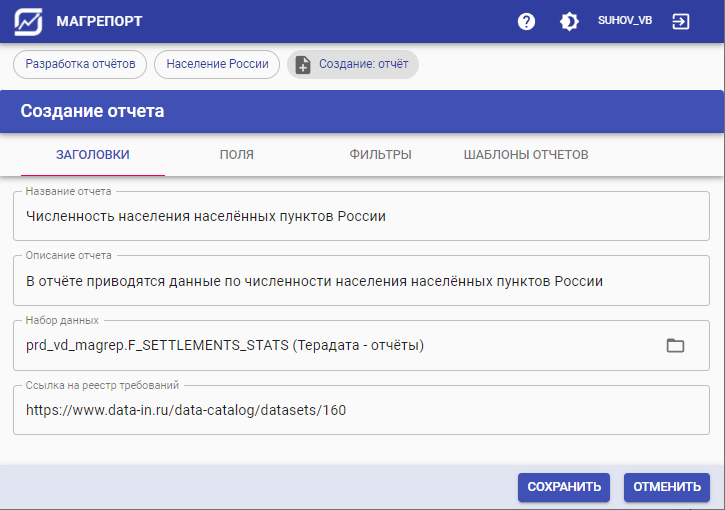
\includegraphics[width=\graphicswidth]{img/5-create-report.png}
		\caption{Дизайнер отчёта}
		\label{fig:create-report}
	\end{figure}

	Дизайнер отчётов состоит из нескольких разделов:
	
	\begin{itemize}
		\item \textbf{Заголовки} (см. рис. \ref{fig:create-report}) --- в этом разделе задаются название отчёта, его краткое описание, указывается набор данных, на котором строится отчёт, и задаётся ссылка на внешнее описание отчёта (называемое, в соответствии с устоявшейся практикой разработчиков системы Магрепорт \textit{реестром требований}). Поле со ссылкой не обязательно для заполнения, если поле оставить незаполненным, кнопка <<Реестр требований>> будет отсутствовать на карточке отчёта.
		
		\item \textbf{Поля} (см. рис. \ref{fig:create-report-fields}) --- в этом разделе редактируются поля отчёта. Поля отчёта формируются из полей набора данных: для каждого поля набора данных указывается выводимое ли оно (кнопка в виде глаза слева от поля), задаётся название поля в отчёте и описание поля (по умолчанию берётся из свойст поля набора данных). Кроме того путём перетаскивания (drag and drop) формируется порядок полей в отчёте.
		
		\item \textbf{Фильтры} (см. рис. \ref{fig:create-report-filters}) --- в этом разделе задаются фильтры отчёта. Формирование фильтров отчёта устроено следюущим образом:
			\begin{itemize}
				\item Фильтры можно объединять в группы. Группы также можно объединять в группы вместе с другими группами или фильтрами. Таким образом фильтры и группы в отчёте образуют иерархическую структуру.
				
				\item Условия, формируемые отдельными фильтрами и группами в рамках объемлющей группы объединяются между собой при помощи логического \textbf{И} или логического \textbf{ИЛИ} --- этим управляет атрибут <<Тип операции>> объемлющей группы. На самом верхнем уровне фильтры и группы объединяются между собой при помощи операции \textbf{И}.
				
				\item Для каждого фильтра и каждой группы фильтров задаются названия, для группы фильтров также задаётся описание. Это просто справочная информация, отображаемая конечному пользователю отчётности.
				
				\item Для каждого фильтра и каждой группы фильтров задаётся обязательный атрибут --- \textit{код}. Этот атрибут участвует только для отчётов на основе хранимых процедур и не имеет значение для отчётов на основе таблиц (или представлений). Подробно вопросы создания отчётов на основе хранимых процедур рассматриваются в разделе \ref{developing:stored-procedure-reports}. Код фильтра по умолчанию берётся из значения атрибута \textit{код} соответствующего экземпляра фильтра (см. раздел \ref{developing:filters}) и может быть изменён. Код группы фильтров формируется по умолчанию случайным образом и может быть изменён. Каждый код должен быть уникален в пределах отчёта.
				
				\item Для каждого фильтра задаётся соответствие полей типа \textit{ID} фильтра с полями отчёта --- таким образом определяется, на какие именно поля набора данных будет накладываться фильтрация в результате применения фильтра. По умолчанию соответствие вычисляется на основе поиска похожих названий полей.
				
				\item Для каждого фильтра и каждой группы фильтров задаётся признак <<Обязательный>> --- обязательный фильтр не может быть оставлен пустым пользователем. В обязательной группе должен быть заполнен хотя бы один фильтр. По умолчанию каждый фильтр добавляется как обязательный.
				
				\item Для каждого фильтров задаётся признак <<Видимый>>. Невидимый фильтр не виден для пользователя и не заполняется им. Невидимые фильтры нужны для того, чтобы распространить действие фильтров безопасности на отчёт в том случае, если пользователю в данном отчёте не требуется явно указывать фильтрацию на основе защищённого справочника. Подробно вопрос фильтров безопасности обсуждаются в главе \ref{administration}. По умолчанию каждый фильтр добавляется как видимый.
				
				\item Порядок следования фильтров и групп не влиет на результирующее условие и может быть изменён методом перетаскивания (drag and drop).
				
			\end{itemize}
		
			\item \textbf{Шаблоны отчётов} --- в этом разделе загружаются и задаются шаблоны отчётов. Шаблоны отчётов могут быть добавлены только при редактировании отчёта. Вопросы создания и загрузки шаблонов отчётов рассмотрены ниже в разделе \ref{developing:customized-excel-templates}.
		
	\end{itemize}

	\begin{figure}[h]
		\centering
		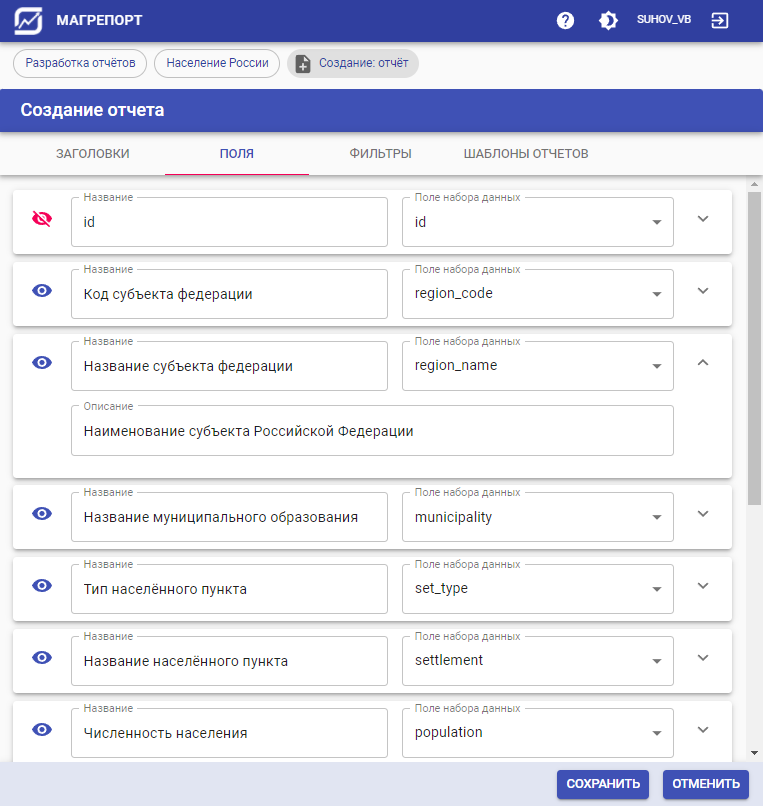
\includegraphics[width=\graphicswidth]{img/6-create-report-fields.png}
		\caption{Дизайнер отчёта --- поля отчёта}
		\label{fig:create-report-fields}
	\end{figure}

	\begin{figure}[h]
		\centering
		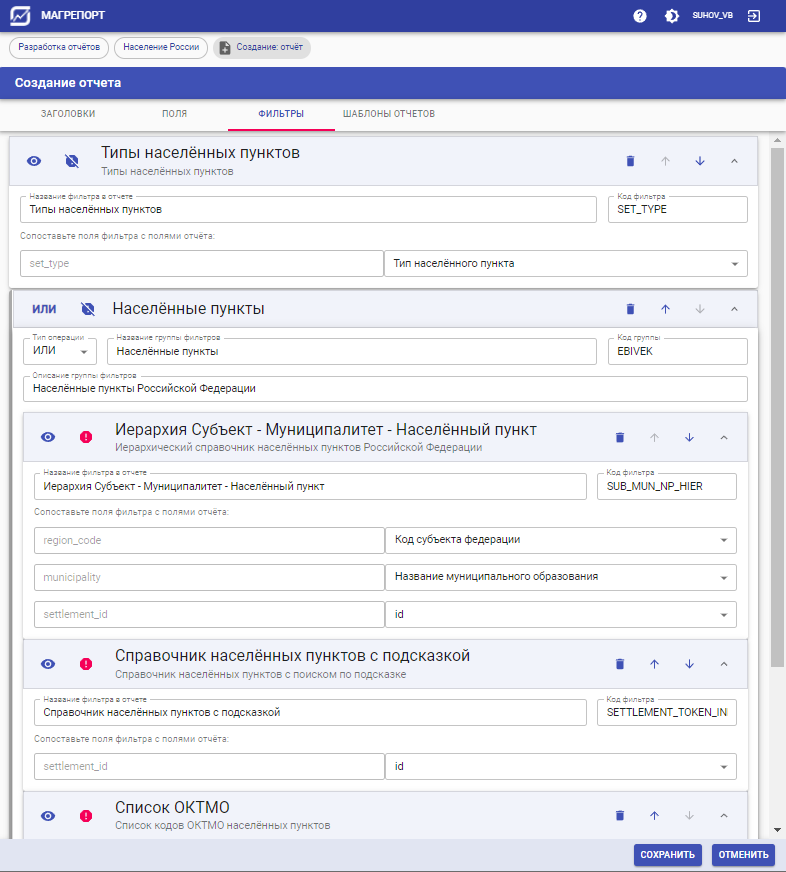
\includegraphics[width=\graphicswidth]{img/7-create-report-filters.png}
		\caption{Дизайнер отчёта --- фильтры}
		\label{fig:create-report-filters}
	\end{figure}

	\begin{devnote}
		Рекомендуется именовать поля фильтра так же, как соответствующие им поля называются в отчёте --- в этом случае соответствие полей фильтра и полей отчёта будет вычисленно автоматически.
	\end{devnote}

	\begin{concept}
		Трудно представить себе отчёт, который бы требовал более одного уровня вложенности групп фильтров (хотя с технической точки зрения ограничений на вложенность групп фильтров никаких нет) --- логика такой фильтрации, скорее всего, будет сложна для восприятия конечным пользователем. Предполагается, что в обычном отчёте фильтры устроены следующим образом: на верхнем уровне идут фильтры по независимым логическим сущностям или по <<\textit{ортогональным}>> измерениям, относящимся к одной и той же сущности: например, идёт фильтр по временн\textit{о}му разрезу, затем фильтр или группа фильтров по географии, затем фильтр или группа фильтром по товарным категориям и фильтр по контрагенту. Такие условия, как правило, требуют объединения через логическое \textbf{И}. В рамках группы, как правило, объединяют фильтры, относящиеся к одной и той же логической сущности, причём к одному и тому же её измерению или <<\textit{сильно связанным}>> измерениям: например, фильтр с географической иерархией, а также фильтр с подсказкой по названию города.
	\end{concept}
	
	\section{Разработка и добавление шаблонов Excel}\label{developing:customized-excel-templates}
	
	Экспорт данных в эксель устроен следующим образом: в выбранном файле шаблона очищается лист с именем \textbf{data} (имя листа задаётся в параметрах приложения --- см. пункт \ref{subsection:excel-template-settings}) и наполняется данным отчёта в виде плоской таблицы с заголовками из названий полей отчёта. Полученный файл в таком виде предоставляется пользователю.
	
	\textit{Стандартный шаблон} (который автоматически добавляется в каждый создаваемый отчёт) устроен следующим образом: он не содержит никаких дополнительных листов, но содержит макрос, формирующий на основые листа \textit{data} сводную таблицу и размещающий её на листе с названием <<Сводная таблица>>. Сводная таблица формируется неразмеченной.
	
	Для данного отчёта можно сделать кастомизированный шаблон, для этого нужно создать чистый файл Excel с поддержкой макросов (имеет расширение xlsm), скопировать в него лист data из выгруженного отчёта, создать все необходимые объекты книги Excel (листы, формулы, макросы, графики), формирующие нужное представление данных на основе листа \textit{data} (см. рис \ref{fig:excel-pivot}), удалить лишние данные с листа \textit{data} (обновив при этом сводные таблицы), чтобы уменьшить размер файла и загрузить шаблон в редакторе отчёта, назвав его подходящим образом (см. рис. \ref{fig:excel-template-uploading}). Шаблон можно отметить как шаблон по умолчанию (см. рис. \ref{fig:set-default-template}) --- в этом случае шаблон будет использоваться по умолчанию для данного отчёта при экспорте. Все лишние шаблоны, в том числе стандартный, можно из отчёта удалить.
	
	\begin{figure}[h]
		\centering
		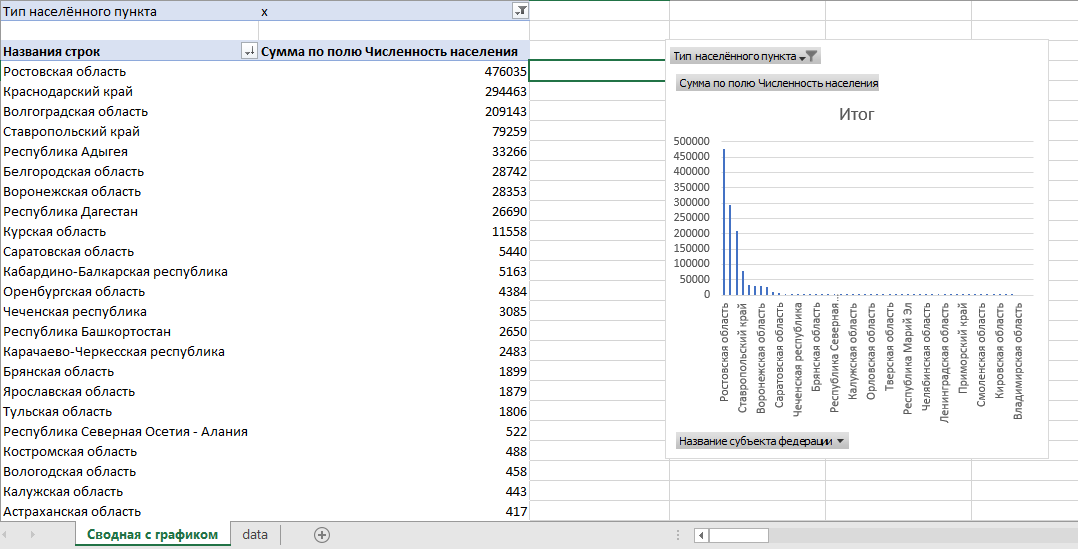
\includegraphics[width=\graphicswidth]{img/14-excel-pivot.png}
		\caption{Пример кастомизированного шаблона}
		\label{fig:excel-pivot}
	\end{figure}	
	
	\begin{figure}[h]
		\centering
		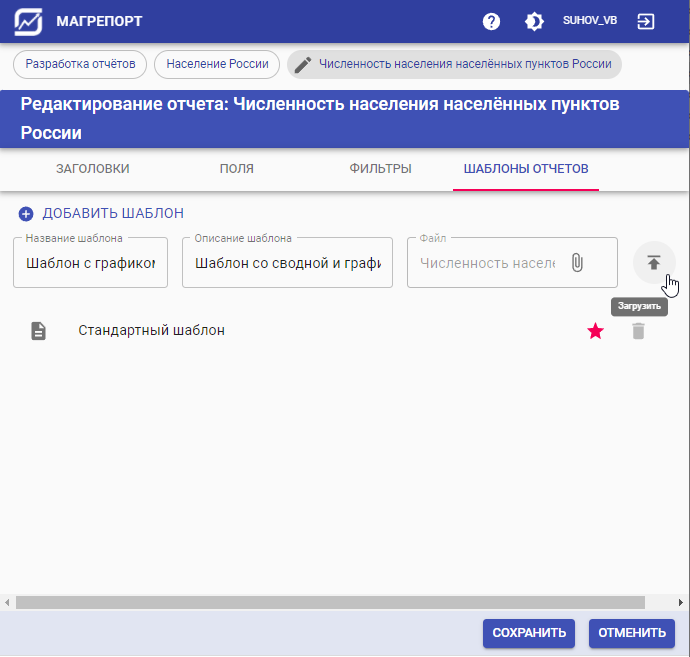
\includegraphics[width=\graphicswidth]{img/15-excel-template-uploading.png}
		\caption{Загрузка кастомизированного шаблона}
		\label{fig:excel-template-uploading}
	\end{figure}	
	
	\begin{figure}[h]
		\centering
		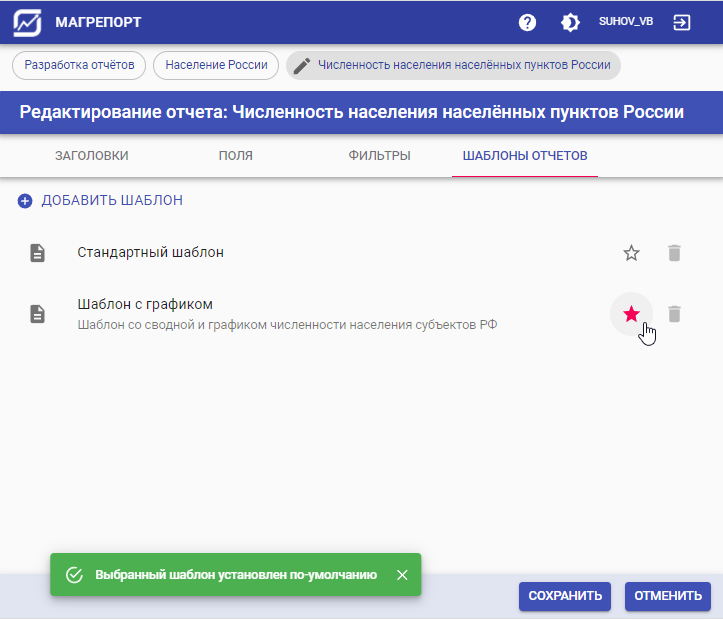
\includegraphics[width=\graphicswidth]{img/16-set-default-template.png}
		\caption{Установка шаблона по умолчанию}
		\label{fig:set-default-template}
	\end{figure}

	\begin{devnote}
		Для сводных таблиц в отчёте рекомендуется устанавливать свойство обновления при открытии файла - см. рис. \ref{fig:excel-pivot-options}.
	\end{devnote}

	\begin{figure}[h]
		\centering
		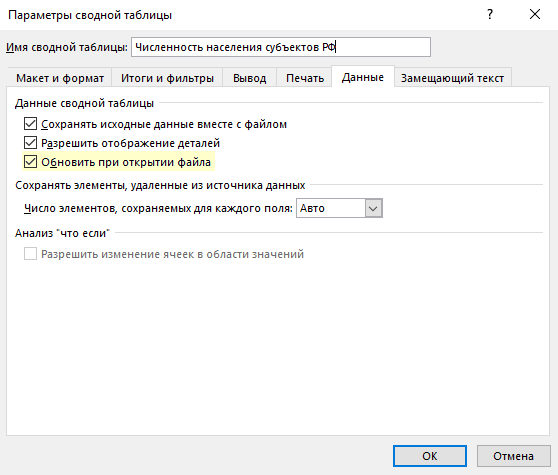
\includegraphics[width=\graphicswidth]{img/13-excel-pivot-options.png}
		\caption{Установка свойства обновления сводной таблицы при открытии файла}
		\label{fig:excel-pivot-options}
	\end{figure}	

	\section{Создание отчётов на хранимых процедурах}\label{developing:stored-procedure-reports}
	
	Наборы данных в системе Магрепорт бывают двух типов: на основе таблиц (или представлений) и на основе хранимых процедур. Отчёты на основе хранимых процедур нужны для реализации сложной внутренней логики отчёта и глубокой оптимизации запросов к БД. Например, запрос требует проброса предиката через подзапрос с аналитической функцией. Через обращение к представлению это невозможно сделать, а без этого запрос будет неэффективен для СУБД. Есть и другие распространнённые примеры, когда необходимо использовать разработку отчёта на основе хранимой процедуры из-за невозможности реализовать логику отчёта в виде представления БД или неэффективности получаемого в итоге запроса.
	
	Разработка отчётов и наборов данных на основе хранимых процедур строится на следующих правилах:
	
	\begin{itemize}
		\item Магрепорт при выполнении отчёта производит вызов хранимой процедуры, передавая ей единственный параметр --- идентификатор задания. Таким образом, каждая такая процедура должна иметь следующую сигнатуру:
		
\begin{lstlisting}[language=SQL]
procedure_name(jobID INTEGER)
\end{lstlisting}
	
	\item Магрепорт в той же схеме, в которой размещается хранимая процедура, создаёт служебные таблицы, в которые записывает значения параметров фильтрации, указанных пользователем. Таким образом, учётной записи, под которой выполняется подключение Магрепорта к БД для данного набора данных, требуются права на создание таблиц и запись данных в таблицы (и чтение данных из таблиц) \textbf{в схеме, в которой размещена хранимая процедура}. Код создаваемых таблиц приведён ниже в листинге \ref{lst:filters-tables}. Реальный DDL-код создаваемых таблиц может варьироваться для различных СУБД с учётом их специфики (например, для Teradata во всех таблицах указывается поле \textit{JOB\_ID} в качестве PRIMARY INDEX).
	
	\item Хранимая процедура должна открывать курсор с данными отчёта в результате своей работы. Результирующий набор данных должен иметь фиксированную структуру. При передаче значения \textbf{NULL} в качестве параметра процедуры (\textbf{jobID}) процедура должна открывать курсор с пустым набором данных такой же структуры --- это требуется для получения Магрепортом информации о полях набора данных при создании набора данных. Структура курсора должна быть фиксированной.
		
	\end{itemize}
	
\begin{lstlisting}[language=SQL, caption={Служебные таблицы для выгрузки параметров фильтрации}, label={lst:filters-tables}]
CREATE TABLE T_REPORT_FILTER
(
	JOB_ID			INTEGER,
	REPORT_FILTER_NAME 	VARCHAR(255),
	FILTER_GROUP_NAME	VARCHAR(255),
	FILTER_TYPE 		VARCHAR(255),
	OPERATION_TYPE 		VARCHAR(255)
);

CREATE TABLE T_REPORT_FILTER_GROUP
(
	JOB_ID 				INTEGER,
	FILTER_GROUP_NAME 		VARCHAR(255),
	PARENT_FILTER_GROUP_NAME	VARCHAR(255),
	GROUP_OPERATION			VARCHAR(255)
);

CREATE TABLE T_REPORT_FILTER_TUPLE
(
	JOB_ID			INTEGER,
	TUPLE_ID		INTEGER,
	REPORT_FILTER_NAME	VARCHAR(255)
);

CREATE TABLE T_REPORT_FILTER_FIELD
(
	JOB_ID 			INTEGER,
	REPORT_FILTER_FIELD_ID	INTEGER,
	TUPLE_ID 		INTEGER,
	FIELD_NAME 		VARCHAR(255)
	DATA_TYPE_FIELD		VARCHAR(255),
	LEVEL 			INTEGER
);

CREATE TABLE T_REPORT_FILTER_FIELD_VALUE
(
	JOB_ID 			INTEGER,
	REPORT_FILTER_FIELD_ID	INTEGER,
	TUPLE_ID 		INTEGER,
	INTEGER_VALUE 		INTEGER,
	DATE_VALUE 		DATE,
	VARCHAR_VALUE 		VARCHAR(255),
	DOUBLE_VALUE 		FLOAT
);
\end{lstlisting}
	
	Приведённые в листинге \ref{lst:filters-tables} служебные таблицы используются в хранимой процедуре для получения значений параметров фильтрации отчёта. Для каждого запуска отчёта в таблицах создаются записи с \textbf{JOB\_ID} равным идентификатору выполняемого задания со следующим содержанием:
	
	\begin{itemize}
		\item \textbf{T\_REPORT\_FILTER} --- фильтры отчёта:
		
			\begin{itemize}
				\item \textit{REPORT\_FILTER\_NAME} --- код фильтра
				\item \textit{FILTER\_GROUP\_NAME} --- код группы фильтров, для корневой группы --- ID отчёта
				\item \textit{FILTER\_TYPE} --- название шаблона фильтра (см. \ref{developing:filters})
				\item \textit{OPERATION\_TYPE} --- тип операции фильтра (\textit{IS\_IN\_LIST}, \textit{IS\_BETWEEN} и т.д.)
			\end{itemize}
		
		\item \textbf{T\_REPORT\_FILTER\_GROUP} --- группы фильтров отчёта:
		
			\begin{itemize}
				\item \textit{FILTER\_GROUP\_NAME} --- код группы фильтров фильтра, для корневой группы --- ID отчёта
				\item \textit{PARENT\_FILTER\_GROUP\_NAME} --- код родительской группы фильтров
				\item \textit{GROUP\_OPERATION} --- логическая операция, применяемая к фильтрам в группе (\textit{AND} или \textit{OR})
			\end{itemize}
		
		\item \textbf{T\_REPORT\_FILTER\_TUPLE} --- список кортежей значений фильтров для данного задания:

			\begin{itemize}
				\item \textit{TUPLE\_ID} --- ID отчёта кортежа
				\item \textbf{REPORT\_FILTER\_NAME} --- код фильтра в отчёте           
			\end{itemize}		
		
		\item \textbf{T\_REPORT\_FILTER\_FIELD} --- связь кортежей и полей фильтров:
	
			\begin{itemize}
				\item \textit{REPORT\_FILTER\_FIELD\_ID} --- ID поля фильтра в отчёте
				\item \textit{TUPLE\_ID} --- ID кортежа
				\item \textit{FIELD\_NAME} --- название поля фильтра в отчёте
				\item \textit{DATA\_TYPE\_FIELD} --- тип значения поля
				\item \textit{LEVEL} --- уровень поля
			\end{itemize}
		
		\item \textbf{T\_REPORT\_FILTER\_FIELD\_VALUE}  --- значения полей фильтров:
			\begin{itemize}
			\item \textit{REPORT\_FILTER\_FIELD\_ID} --- ID поля фильтра в отчёте
			\item \textit{TUPLE\_ID} --- ID кортежа
			\item \textit{INTEGER\_VALUE} --- значение поля для целочисленных полей
			\item \textit{DATE\_VALUE} --- значение поля для полей типа DATE
			\item \textit{VARCHAR\_VALUE} --- значение поля для полей типа VARCHAR
			\item \textit{DOUBLE\_VALUE} --- значение поля для полей типа FLOAT
		\end{itemize}
		
	\end{itemize}

	Значения, указанные пользователем в фильтрах, образуют кортежи --- у каждого кортежа на данном уровне одно значение. Кортеж может содержать один или несколько уровней. Одноуровневые кортежи значений получаются в результате выбора значений в таких фильтрах, в которых каждый отдельный выбор пользователя описывается одним атомарным значением (то есть является либо числом, либо строкой, либо датой) --- как, например, в фильтрах типа VALUE\_LIST или TOKEN\_INPUT. Многоуровневые кортежи получаются в результате таких выборов пользователя, которые описываются несколькими атомарными значениями --- как, например, в фильтрах типа DATE\_RANGE (один выбор --- это два значения --- <<дата с>> и <<дата по>>) или иерархических фильтрах (каждый выборанный узел описывается целым кортежем значений идентификаторов всех узлов с первого уровня иерархии вплоть до данного). Перечень кортежей для данного фильтра представлен в таблице \textit{T\_REPORT\_FILTER\_TUPLE}, разбивка по уровням и привязка к конкретному полю фильтра указана в таблице \textit{T\_REPORT\_FILTER\_FIELD}, конкретные значения кортежей, соответствующие данному полю, указаны в таблице \textit{T\_REPORT\_FILTER\_FIELD\_VALUE}.
	
	Для получения указанных пользователем значений фильтров и их соответствия фильтрам и полям фильтров можно воспользоватся представлением, указанным в листинге \ref{lst:report-filter-value-view} (представление не создаётся автоматически --- разработчики могут создать его самостоятельно).
	
	
\begin{lstlisting}[language=SQL, caption={Представление для получения значений выбора в фильтрах}, label={lst:report-filter-value-view}]
CREATE VIEW V_REPORT_FILTER_VALUE
as
SELECT 
	rf.JOB_ID	
	, rf.REPORT_FILTER_NAME 
	, rf.FILTER_TYPE
	, rft.TUPLE_ID	
	, rff.FIELD_NAME
	, rff.LEVEL as FIELD_LEVEL 
	, rffv.INTEGER_VALUE                 
	, rffv.DATE_VALUE                    
	, rffv.VARCHAR_VALUE                 
	, rffv.DOUBLE_VALUE            
FROM T_REPORT_FILTER rf 
    inner join T_REPORT_FILTER_TUPLE rft on 
    	rf.JOB_ID = rft.JOB_ID
	    and rf.REPORT_FILTER_NAME = rft.REPORT_FILTER_NAME
    inner join T_REPORT_FILTER_FIELD rff on 
    	rff.JOB_ID = rf.JOB_ID
   	    and rff.TUPLE_ID = rft.TUPLE_ID	
    inner join T_REPORT_FILTER_FIELD_VALUE rffv on 
    	rffv.JOB_ID = rf.JOB_ID
	    and rffv.REPORT_FILTER_FIELD_ID = 
	    	rff.REPORT_FILTER_FIELD_ID
	    and rffv.TUPLE_ID = rff.TUPLE_ID
\end{lstlisting}

	На основе представления, представленного в листинге \ref{lst:report-filter-value-view}, разработчики могут создать систему представлений, предназначенных для получения значения конкретного фильтра в удобном виде и далее использовать его для соединения с таблицами фактов или справочников. Это и есть основа для разработки отчётов на основе хранимых процедур для системы Магрепорт.
	
	Важно: при получении значений по коду фильтра возвращаются только значения, непосредственно указанные пользователем в фильтре, значения ограничений из фильтров безопасности не возвращаются. Если в отчёте присуствуют фильтры, защищённые фильтрами безопасности, дополнительно в таблицы со значениями фильтров пользователя выгружаются ограничения фильтров безопасности, соответствующие пользователю. При этом к коду фильтра добавляется префикс <<SF\_>>.
	
	\begin{devnote}
		Не рекомендуется давать коды фильтрам, начинающиеся с префикса <<SF\_>>, чтобы отличать значения фильтров, заданные пользователями, от значений фильтров безопасности.
	\end{devnote}

	Одним из возможных рекомендованных подходов к разработке хранимых процедур является создание служебных вспомогательных процедур, наполняющих временные (или постоянные) таблицы с ключами сущностей, по которым строится отчёт. Эти процедуры должны учитывать возможные фильтры и фильтры безопасности для данных сущностей. После этого сформированный список ключей разработчик может использовать в основной процедуре.

	\section{Обновление наборов данных}
	
	Может возникнуть ситуация, при которой в наборе данных обновится состав полей или их типы. В этом случае необходимо выполнить обновление набора данных. Для этого нужно зайти в набор данных в режиме редактирования и в разделе <<Поля>> в левом верхнем углу нажать кнопку <<Обновить>> (см. рис. \ref{fig:update-fields-button}).
		
	\begin{figure}[h]
		\centering
		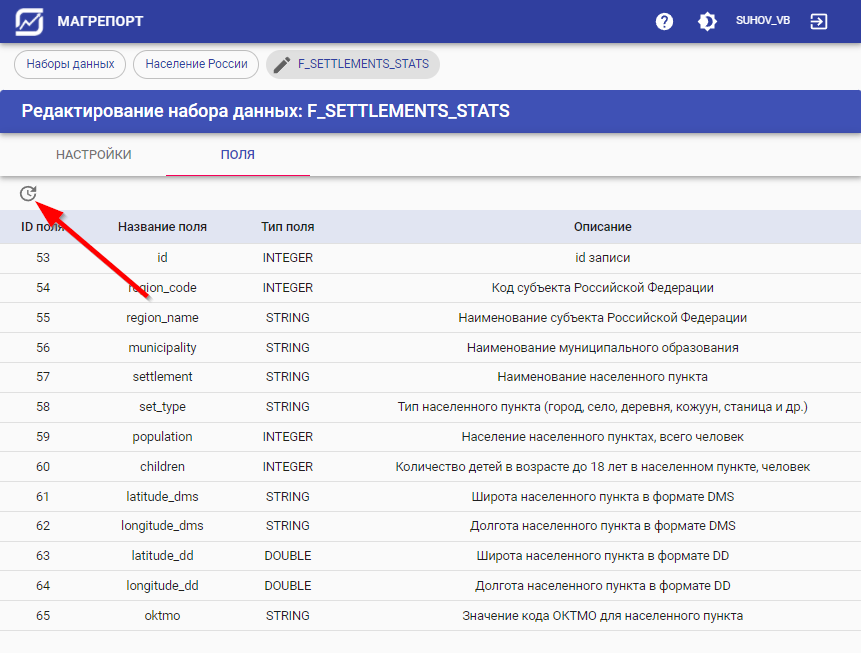
\includegraphics[width=\graphicswidth]{img/8-update-fields-button.png}
		\caption{Кнопка обновления полей}
		\label{fig:update-fields-button}
	\end{figure}

	При обновлении набора данных происходит следующее:
	\begin{itemize}
		\item добавляются новые поля набора данных;
		\item удаляются отсуствующие поля набора данных;
		\item обновляются типы данных полей.
	\end{itemize}
	При этом может возникнуть ситуация, когда просто так нельзя удалить поле набора данных в силу того, что оно используется в зависимом объекте (фильтре или отчёте). В этом случае такое поле помечается красным как несуществующие (см. рис. \ref{fig:update-fields-invalid-field}), а сам набор данных помечается как невалидный и его карточка тоже становится красной (см. рис. \ref{fig:invalid-dataset}). Также невалидными становятся все объекты, зависящие от данного набора данных: фильтры и отчёты (их карточки также становятся красными). Свойство невалидности рекурсивно распространяется на зависимые объекты (если фильтр стал невалидным, то невалидными становятся и отчёты, содержащие фильтр). Свойство невалидности не мешает использовать объекты, однако сигнализирует о том, что есть проблема, которая может привести к неправильной работе объекта. Получить список зависимых объектов можно при помощи кнопки <<Показать зависимости>> в левом нижнем углу карточки объекта (см. рис. \ref{fig:show-dependencies-button}).
	
	\begin{figure}[h]
		\centering
		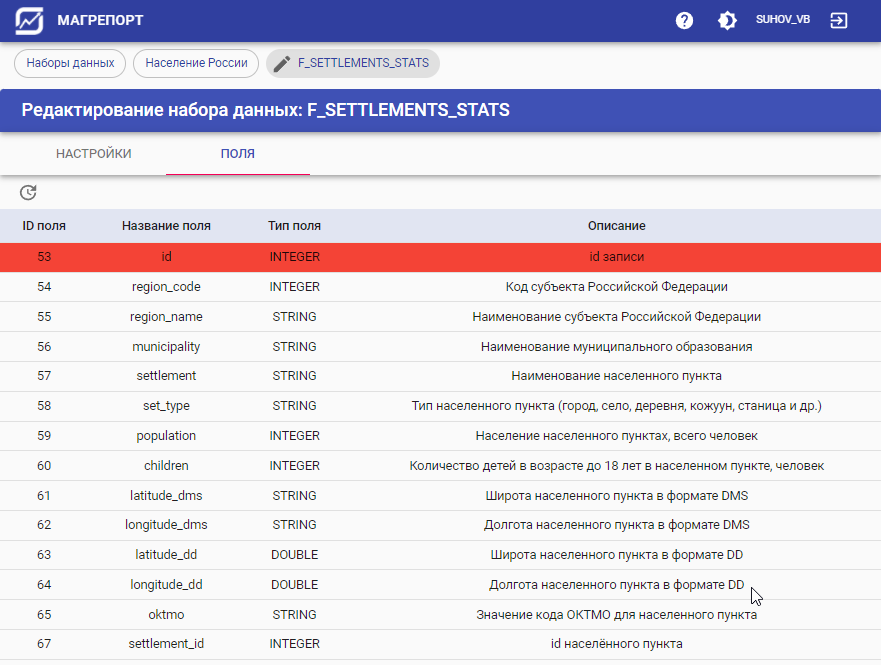
\includegraphics[width=\graphicswidth]{img/9-update-fields-invalid-field.png}
		\caption{Невалидное поле в наборе данных}
		\label{fig:update-fields-invalid-field}
	\end{figure}	

	\begin{figure}[h]
		\centering
		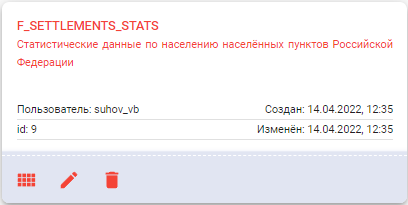
\includegraphics[width=\graphicswidth]{img/10-invalid-dataset.png}
		\caption{Невалидный набор данных}
		\label{fig:invalid-dataset}
	\end{figure}	

	Чтобы исправить невалидность объекта нужно в зависимых фильтрах изменить зависимость от невалидного поля на зависимость от валидного поля, в отчётах в списке полей удалить невалидное поле (у невалидных полей появится кнопка удаления - см. рис. \ref{fig:delete-field-button}) и в разделе <<Фильтры>> перенастроить все фильтры так, чтобы они не использовали невалидное поле. Если зависимость от невалидного поля устраняется, объект становится валидным.

	\begin{figure}[h]
		\centering
		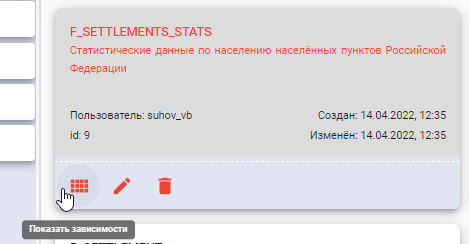
\includegraphics[width=\graphicswidth]{img/11-show-dependencies-button.png}
		\caption{Кнопка <<Показать зависимости>>}
		\label{fig:show-dependencies-button}
	\end{figure}	

	\begin{figure}[h]
		\centering
		
\includegraphics[width=\graphicswidth]{img/12-delete-field-button.png}
		\caption{Кнопка удаления невалидного поля}
		\label{fig:delete-field-button}
	\end{figure}	
	
	После того, как все зависимые объекты исправлены, необходимо снова зайти в набор данных и выполнить обновление полей. Если от удалённого поля больше никакой объект не зависит, оно пропадёт после обновления из списка полей и набор данных станет валидным.

	\section{Публикация отчётов}\label{developing:publishing-report}
	
	В системе Магрепорт дерево каталогов разработки отчётов и дерево пользовательских каталогов, в которых конечные пользователи видят отчёты для запуска, существуют независимо друг от друга. Разработчики и администраторы системы могут конвенционально поддерживать взаимное соответствие их структур, либо не стремиться к этому (например, разделяя каталоги разработки отчётов по командам разработки, а пользовательские каталоги --- по предметной области отчёта).
	
	Для предоставления доступа к отчёту конечным пользователям, отчёт необходимо \textit{опубликовать} в пользовательском каталоге (раздел меню <<Отчёты>>). Для публикации отчёта нужно иметь права на запись в каталог публикации и права на чтение к каталогу разработки, в котором размещён отчёт. Для выполнения публикации нужно нажать кнопку <<Добавить>> в правом нижнем углу экрана, выбрать пункт <<Добавить отчёт>> (см. рис. \ref{fig:publishing-report}) и в появившемся окне навигации выбрать соответствующий отчёт (см. рис. \ref{fig:navigate-to-report}). Отчёт (фактически ссылка на отчёт) будет добавлен в текущий каталог.
	
	\begin{figure}[h]
		\centering
		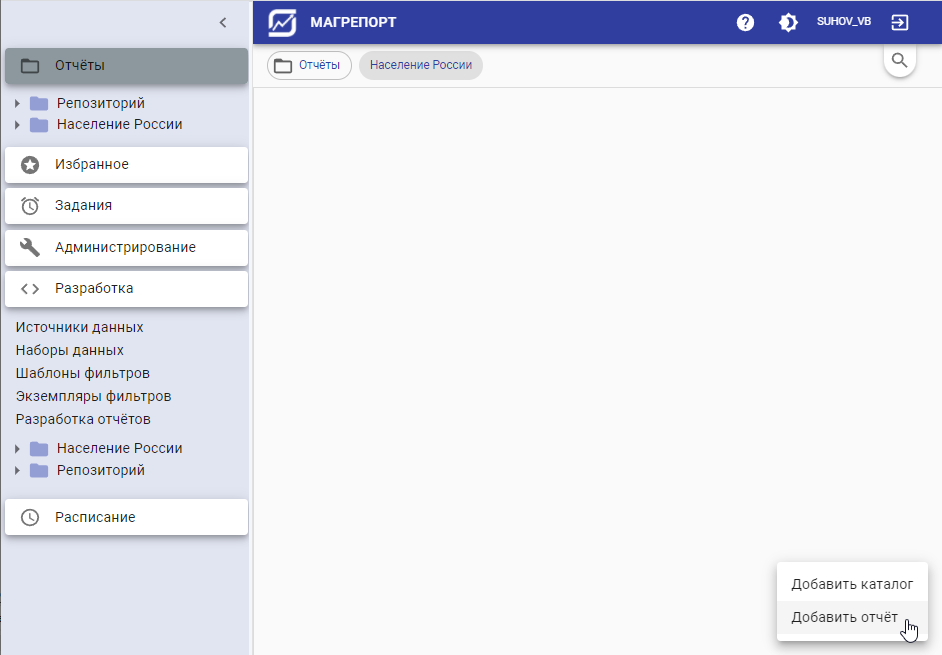
\includegraphics[width=\graphicswidth]{img/17-publishing-report.png}
		\caption{Публикация отчёта}
		\label{fig:publishing-report}
	\end{figure}		

	\begin{figure}[h]
		\centering
		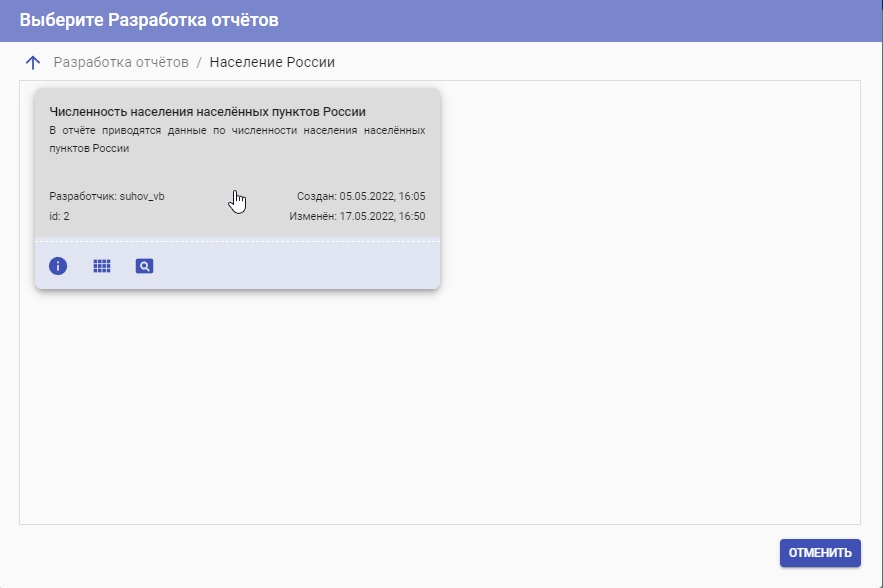
\includegraphics[width=\graphicswidth]{img/18-navigate-to-report.png}
		\caption{Выбор отчёта в окне навигации}
		\label{fig:navigate-to-report}
	\end{figure}	

	По причине того, что в пользовательских каталогах фактически размещаются ссылки на отчёты, в системе не реализована возможность копировать и переносить эти ссылки между каталогами. Для реализации этой потребности можно просто добавить ссылку в другой каталог и при необходимости удалить ссылку из данного. Создать две ссылки на один и тот же отчёт в одном и том же пользовательском каталоге нельзя.
	
\end{document}